% Created by tikzDevice version 0.12.6 on 2026-08-03 04:28:50
% !TEX encoding = UTF-8 Unicode
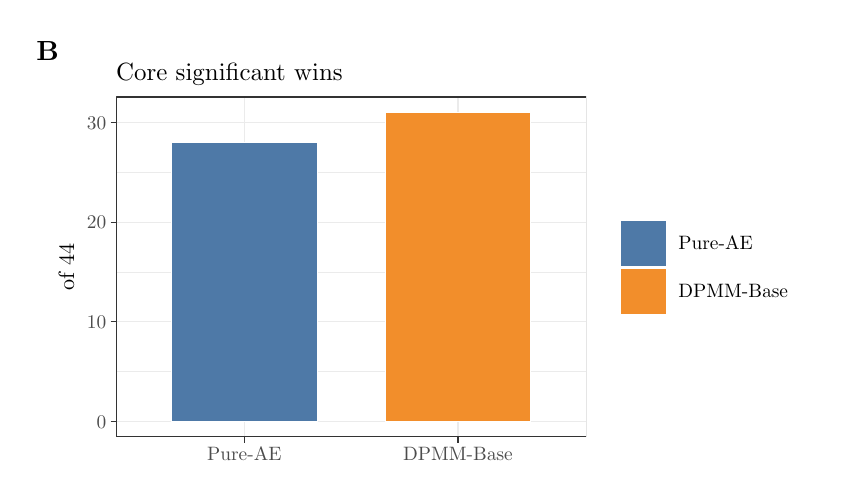
\begin{tikzpicture}[x=1pt,y=1pt]
\definecolor{fillColor}{RGB}{255,255,255}
\path[use as bounding box,fill=fillColor,fill opacity=0.00] (0,0) rectangle (283.84,161.83);
\begin{scope}
\path[clip] (  1.11,  1.74) rectangle (282.74,160.09);
\definecolor{drawColor}{RGB}{255,255,255}
\definecolor{fillColor}{RGB}{255,255,255}

\path[draw=drawColor,line width= 0.4pt,line join=round,line cap=round,fill=fillColor] (  1.11,  1.74) rectangle (282.74,160.09);
\end{scope}
\begin{scope}
\path[clip] ( 31.98, 13.93) rectangle (201.81,136.79);
\definecolor{fillColor}{RGB}{255,255,255}

\path[fill=fillColor] ( 31.98, 13.93) rectangle (201.81,136.79);
\definecolor{drawColor}{gray}{0.92}

\path[draw=drawColor,line width= 0.2pt,line join=round] ( 31.98, 37.53) --
	(201.81, 37.53);

\path[draw=drawColor,line width= 0.2pt,line join=round] ( 31.98, 73.56) --
	(201.81, 73.56);

\path[draw=drawColor,line width= 0.2pt,line join=round] ( 31.98,109.59) --
	(201.81,109.59);

\path[draw=drawColor,line width= 0.4pt,line join=round] ( 31.98, 19.52) --
	(201.81, 19.52);

\path[draw=drawColor,line width= 0.4pt,line join=round] ( 31.98, 55.55) --
	(201.81, 55.55);

\path[draw=drawColor,line width= 0.4pt,line join=round] ( 31.98, 91.58) --
	(201.81, 91.58);

\path[draw=drawColor,line width= 0.4pt,line join=round] ( 31.98,127.60) --
	(201.81,127.60);

\path[draw=drawColor,line width= 0.4pt,line join=round] ( 78.29, 13.93) --
	( 78.29,136.79);

\path[draw=drawColor,line width= 0.4pt,line join=round] (155.49, 13.93) --
	(155.49,136.79);
\definecolor{drawColor}{RGB}{255,255,255}
\definecolor{fillColor}{RGB}{242,142,43}

\path[draw=drawColor,line width= 0.3pt,fill=fillColor] (129.24, 19.52) rectangle (181.74,131.21);
\definecolor{fillColor}{RGB}{78,121,167}

\path[draw=drawColor,line width= 0.3pt,fill=fillColor] ( 52.05, 19.52) rectangle (104.54,120.40);
\definecolor{drawColor}{gray}{0.20}

\path[draw=drawColor,line width= 0.4pt,line join=round,line cap=round] ( 31.98, 13.93) rectangle (201.81,136.79);
\end{scope}
\begin{scope}
\path[clip] (  0.00,  0.00) rectangle (283.84,161.83);
\definecolor{drawColor}{gray}{0.30}

\node[text=drawColor,anchor=base east,inner sep=0pt, outer sep=0pt, scale=  0.70] at ( 28.38, 17.11) {0};

\node[text=drawColor,anchor=base east,inner sep=0pt, outer sep=0pt, scale=  0.70] at ( 28.38, 53.14) {10};

\node[text=drawColor,anchor=base east,inner sep=0pt, outer sep=0pt, scale=  0.70] at ( 28.38, 89.16) {20};

\node[text=drawColor,anchor=base east,inner sep=0pt, outer sep=0pt, scale=  0.70] at ( 28.38,125.19) {30};
\end{scope}
\begin{scope}
\path[clip] (  0.00,  0.00) rectangle (283.84,161.83);
\definecolor{drawColor}{gray}{0.20}

\path[draw=drawColor,line width= 0.4pt,line join=round] ( 29.98, 19.52) --
	( 31.98, 19.52);

\path[draw=drawColor,line width= 0.4pt,line join=round] ( 29.98, 55.55) --
	( 31.98, 55.55);

\path[draw=drawColor,line width= 0.4pt,line join=round] ( 29.98, 91.58) --
	( 31.98, 91.58);

\path[draw=drawColor,line width= 0.4pt,line join=round] ( 29.98,127.60) --
	( 31.98,127.60);
\end{scope}
\begin{scope}
\path[clip] (  0.00,  0.00) rectangle (283.84,161.83);
\definecolor{drawColor}{gray}{0.20}

\path[draw=drawColor,line width= 0.4pt,line join=round] ( 78.29, 11.93) --
	( 78.29, 13.93);

\path[draw=drawColor,line width= 0.4pt,line join=round] (155.49, 11.93) --
	(155.49, 13.93);
\end{scope}
\begin{scope}
\path[clip] (  0.00,  0.00) rectangle (283.84,161.83);
\definecolor{drawColor}{gray}{0.30}

\node[text=drawColor,anchor=base,inner sep=0pt, outer sep=0pt, scale=  0.70] at ( 78.29,  5.51) {Pure-AE};

\node[text=drawColor,anchor=base,inner sep=0pt, outer sep=0pt, scale=  0.70] at (155.49,  5.51) {DPMM-Base};
\end{scope}
\begin{scope}
\path[clip] (  0.00,  0.00) rectangle (283.84,161.83);
\definecolor{drawColor}{RGB}{0,0,0}

\node[text=drawColor,rotate= 90.00,anchor=base,inner sep=0pt, outer sep=0pt, scale=  0.80] at ( 16.80, 75.36) {of 44};
\end{scope}
\begin{scope}
\path[clip] (  0.00,  0.00) rectangle (283.84,161.83);
\definecolor{fillColor}{RGB}{255,255,255}

\path[fill=fillColor] (209.81, 54.02) rectangle (280.74, 96.71);
\end{scope}
\begin{scope}
\path[clip] (  0.00,  0.00) rectangle (283.84,161.83);
\definecolor{fillColor}{RGB}{255,255,255}

\path[fill=fillColor] (213.81, 75.36) rectangle (231.15, 92.71);
\definecolor{drawColor}{RGB}{255,255,255}
\definecolor{fillColor}{RGB}{78,121,167}

\path[draw=drawColor,line width= 0.3pt,fill=fillColor] (214.17, 75.72) rectangle (230.80, 92.35);
\end{scope}
\begin{scope}
\path[clip] (  0.00,  0.00) rectangle (283.84,161.83);
\definecolor{fillColor}{RGB}{255,255,255}

\path[fill=fillColor] (213.81, 58.02) rectangle (231.15, 75.36);
\definecolor{drawColor}{RGB}{255,255,255}
\definecolor{fillColor}{RGB}{242,142,43}

\path[draw=drawColor,line width= 0.3pt,fill=fillColor] (214.17, 58.37) rectangle (230.80, 75.01);
\end{scope}
\begin{scope}
\path[clip] (  0.00,  0.00) rectangle (283.84,161.83);
\definecolor{drawColor}{RGB}{0,0,0}

\node[text=drawColor,anchor=base west,inner sep=0pt, outer sep=0pt, scale=  0.70] at (235.15, 81.62) {Pure-AE};
\end{scope}
\begin{scope}
\path[clip] (  0.00,  0.00) rectangle (283.84,161.83);
\definecolor{drawColor}{RGB}{0,0,0}

\node[text=drawColor,anchor=base west,inner sep=0pt, outer sep=0pt, scale=  0.70] at (235.15, 64.28) {DPMM-Base};
\end{scope}
\begin{scope}
\path[clip] (  0.00,  0.00) rectangle (283.84,161.83);
\definecolor{drawColor}{RGB}{0,0,0}

\node[text=drawColor,anchor=base west,inner sep=0pt, outer sep=0pt, scale=  0.90] at ( 31.98,142.78) {Core significant wins};
\end{scope}
\begin{scope}
\path[clip] (  0.00,  0.00) rectangle (283.84,161.83);
\definecolor{drawColor}{RGB}{0,0,0}

\node[text=drawColor,anchor=base,inner sep=0pt, outer sep=0pt, scale=  1.00] at (  7.20,150.08) {\bfseries B};
\end{scope}
\end{tikzpicture}
